\section{Transverse Shear}

Transverse loading creates corresponding \textbf{longitudinal shear stresses} which will act along longitudinal planes of the beam

\begin{figure*}[!h]
\centering
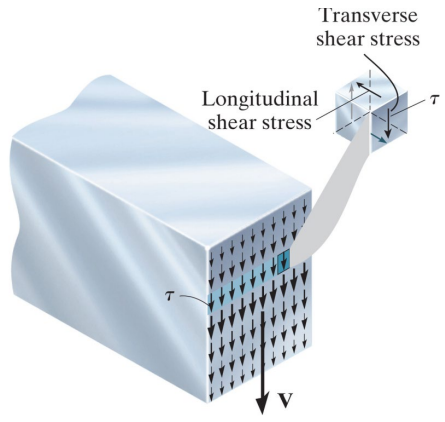
\includegraphics[angle=0, width=2in]{TransverseShear-Figures/TransToLong.png}
\vspace{-2mm}
\caption{\small \cyan{Taken from the web}}
\vspace{-3mm}
\label{Fig:TransToLong}
\end{figure*}

\subsection{\blue{Shear Stress in Beams}}

\begin{figure*}[!h]
\centering
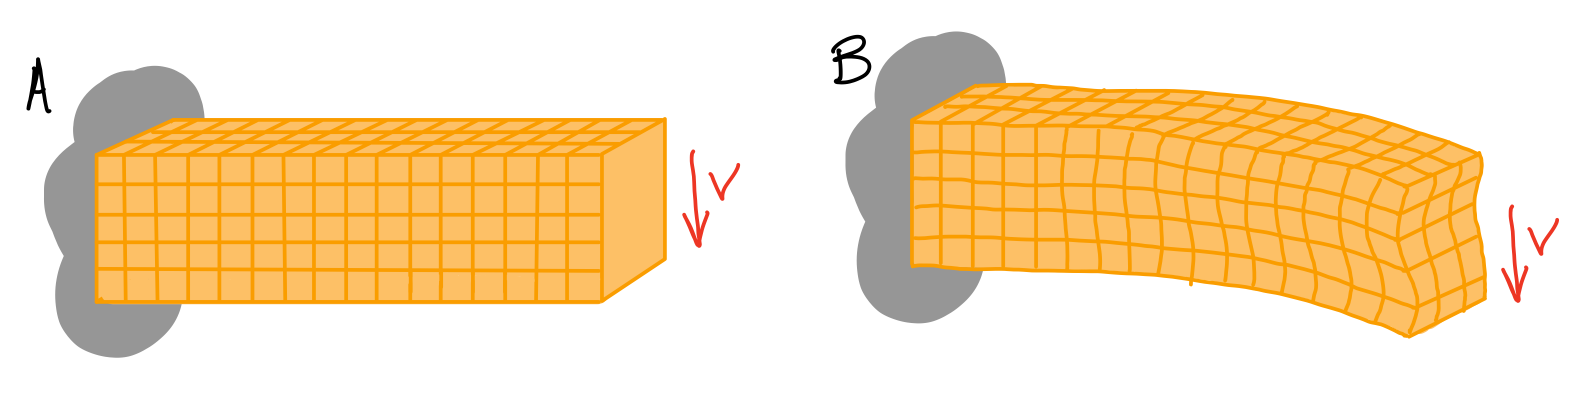
\includegraphics[angle=0, width=2.5in]{TransverseShear-Figures/TransverseShear.png}
\vspace{-2mm}
\caption{\small \blue{Taken from TAM251 Lecture Notes - L7S3}}
\vspace{-3mm}
\label{Fig:MaxStress}
\end{figure*}

\noindent When a shear force is applied, it tends to cause warping of the cross section. Therefore, when a beam is subject to moments and shear forces, the \textbf{cross section will not remain plane} as assumed in the derivation of the flexural formula. However, we can assume that the warping due to shear is small enough to be neglected, which is particularly true for slender beams.

\vspace{5pt}

\noindent \textbf{\red{**Reference pages have a broken link image here**}} 

\begin{figure*}[!h]
\centering
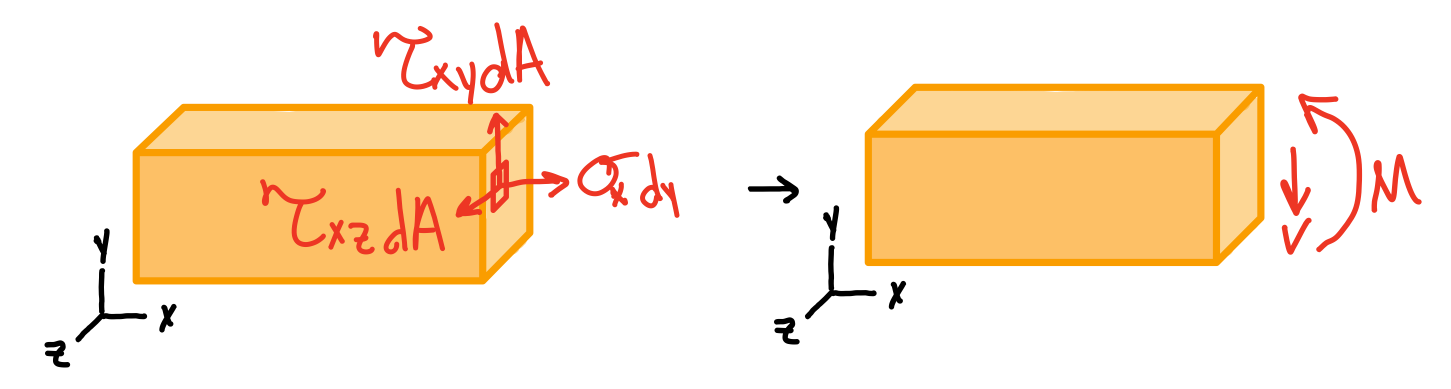
\includegraphics[angle=0, width=3in]{TransverseShear-Figures/EquilibriumEqtn.png}
\vspace{-2mm}
\caption{\small \cyan{Taken from the web}}
\vspace{-3mm}
\label{Fig:EquilEqtn}
\end{figure*}

\noindent Transverse loading applied to a beam results in normal and shearing stresses in transverse sections\cyan{, as well as a bending moment}.

\vspace{5pt}

\noindent The distribution of normal and shearing stresses satisfies:

\[
\begin{align*}
&F_x = \int\sigma_x dA = 0 		 &M_x &= \int(y\tau_{xz} - z\tau_{xy})dA=0 \\
&F_y = \int\tau_{xy} dA = -V 	 &M_y &= \int z\sigma_{x} dA = 0 \\
&F_z = \int\tau_{xz} dA = 0 	 &M_z &= \int(-y\sigma_{x})dA = M \\
\end{align*}
\]

\noindent When shearing stresses are exerted on the vertical faces of an element, equal stresses must be exerted on the horizontal faces.

\vspace{5pt}

\noindent Longitudinal shearing stresses must exist in any member subjected to transverse loading.

\vspace{5pt}

\noindent Symmetry of stress: transverse xy stress implies longitudinal yx stress

\[\tau_{xy} = \tau_{yx}\]

\vspace{5pt}

\noindent \textbf{\red{**Reference pages have a broken link image here**}} 

\begin{figure*}[!h]
\centering
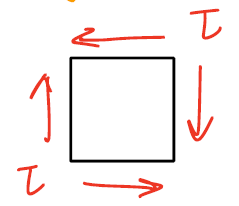
\includegraphics[angle=0, width=2in]{TransverseShear-Figures/Symmetry.png}
\vspace{-2mm}
\caption{\small \blue{Guessed based on context clues and lecture slides}}
\vspace{-3mm}
\label{Fig:Symmetry}
\end{figure*}
 
\subsection{\blue{Average Shear Stress}}

\begin{figure*}[!h]
\centering
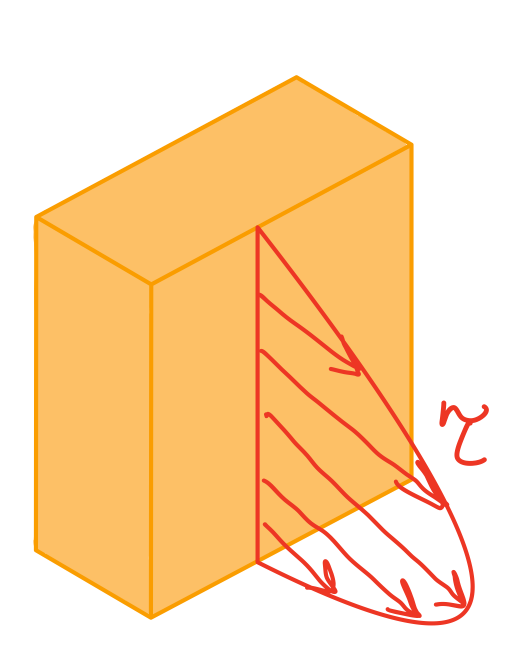
\includegraphics[angle=0, width=\columnwidth]{TransverseShear-Figures/AvgShear.png}
\vspace{-2mm}
\caption{\small \blue{Taken from TAM251 Lecture Notes - L7S6-7}}
\vspace{-3mm}
\label{Fig:AvgShear}
\end{figure*}

\noindent \blue{Average shear stress is given by \[\tau = \frac{V}{A}\]}

\noindent \blue{Shear stress at a specific point is given by \[\tau = \frac{VQ}{It}\]}

\blue{
\begin{itemize}
    \item $V$: shear force
    \item $Q$: First area moment of inertia of cut section ($Q = \Sigma yA$)
    \item $I$: Second area moment of inertia of whole section
    \item $t$: beam thickness
\end{itemize}
}


\noindent \cyan{\textbf{**Expandable Derivation**}}

\begin{figure*}[!h]
\centering
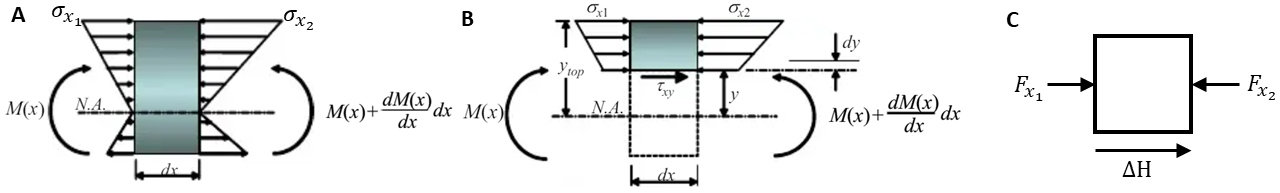
\includegraphics[angle=0, width=\columnwidth]{TransverseShear-Figures/ElementFBD.png}
\vspace{-2mm}
\caption{\small \cyan{Taken from the web}}
\vspace{-3mm}
\label{Fig:EquilEqtn}
\end{figure*}

\noindent \cyan{\textbf{(A)} An element of width $dx$ in a bending beam has a FBD of the bending moment stress distribution.}

\vspace{5pt}

\noindent \cyan{\textbf{(B)} An element distance $y$ away from the neutral axis has a FBD of the bending moment stress distribution For this element to be in equilibrium, $\tau_{xy}$ must be present.}

\cyan{\[\sigma_{x_1} \neq \sigma_{x_2}\]}

\noindent \cyan{\textbf{(C)} Simplified FBD. The width of this element is $t(y)$.}

\cyan{
\[F_x = \int\sigma_x dA = 0\]
\[\Sigma F_x = F_{x_1} - F_{x_2} + \Delta H\]
\[\int_{y}^{y_{top}} \sigma_{x_1} t(y) dy - \int_{y}^{y_{top}} \sigma_{x_2} t(y) dy + \tau_{xy} t(y) dx = 0\]
\[\int_{y}^{y_{top}} \frac{M(x)y}{I} t(y) dy - \int_{y}^{y_{top}} \frac{(M(x)+dM(x))y}{I} t(y) dy + \tau_{xy} t(y) dx = 0\]
\[\tau_{xy} = \frac{dM(x)}{dx}\frac{1}{I t(y)} \int_{y}^{y_{top}} y t(y) dy\]
\[V(x) = \frac{dM(x)}{dx}\]
\[\tau_{xy} = \frac{V(x)}{I t(y)} \int_{y}^{y_{top}} y t(y) dy\]
\[\tau_{xy} = \frac{V(x) Q(y)}{I t(y)}\]
}

\noindent \cyan{\textbf{**End Derivation**}}

\subsubsection{\blue{Rectangular Beam Cross-Section}}

\begin{figure*}[!h]
\centering
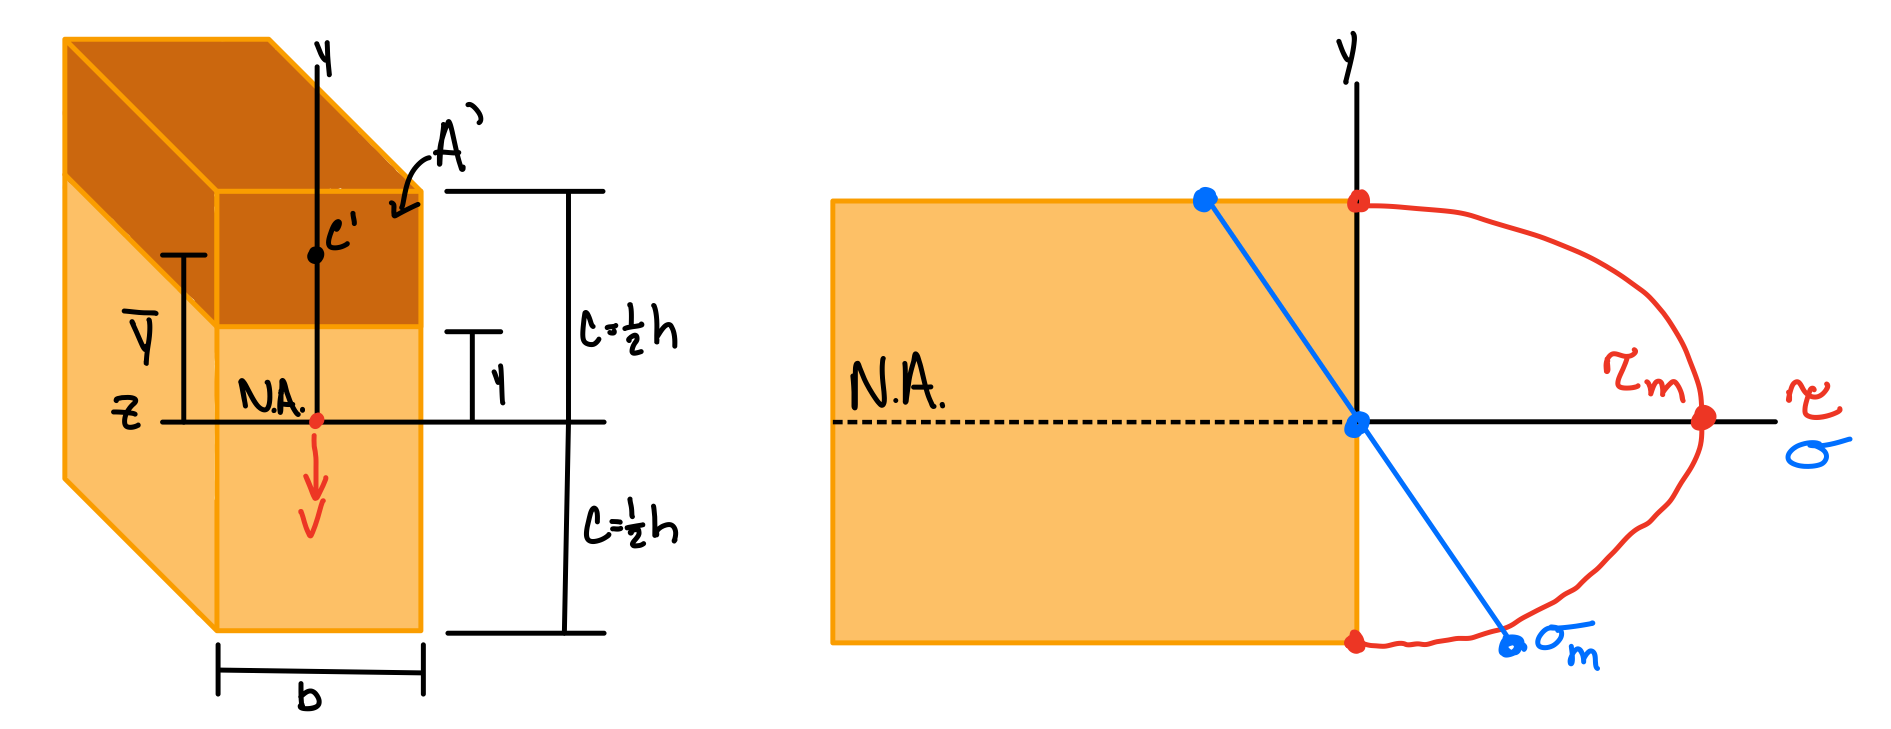
\includegraphics[angle=0, width=5in]{TransverseShear-Figures/RectCrossSect.png}
\vspace{-2mm}
\caption{\small \blue{Taken from TAM251 Lecture Notes - L7S8}}
\vspace{-3mm}
\label{Fig:RectCrossSect}
\end{figure*}

\blue{
\[\tau = \frac{3}{2} \frac{V}{bh}(1-\frac{y^2}{c^2})\]
where \[c = \frac{1}{2}h\]
}

\noindent \cyan{or
\[\tau = \frac{6V}{bh^3}(\frac{h^2}{4}-y^2)\]
}
\noindent \blue{\textbf{**Expandable Derivation**}}
\blue{
\[I_z = \frac{1}{12} bh^3\]
\[t=b\]
\[Q = A\bar{y}\]
\[Q = b(\frac{1}{2}h-y)[y+\frac{1}{2}(\frac{1}{2}h-y)]\]
\[Q = \frac{1}{2}b(\frac{1}{4}h^2-y^2)\]
}
\noindent \blue{\textbf{**End Derivation**}}

\vspace{5pt}
 
\noindent \cyan{Maximum shear stress occurs at the Neutral axis
\[\tau_{max} = 1.5 \frac{V}{A}\]
}

\vspace{5pt}

\noindent Anisotropic material: wood fails at locations of maximum longitudinal stress

\vspace{5pt}

\noindent \textbf{\red{**Reference pages have a broken link image here**}} 

\subsubsection{\blue{I-Shaped Beam Cross-Section}}

\begin{figure*}[!h]
\centering
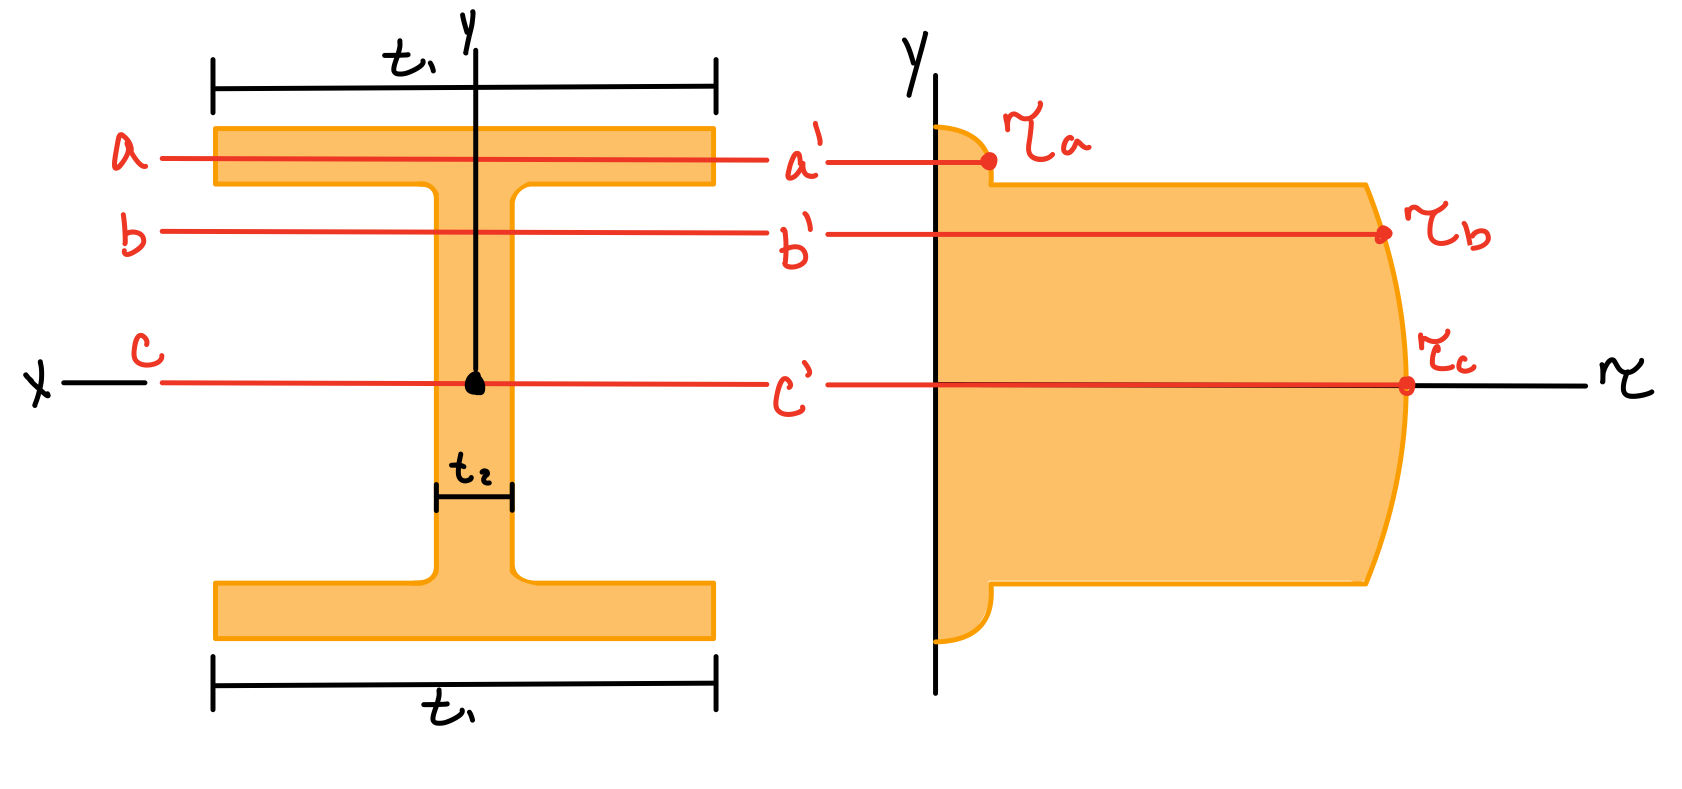
\includegraphics[angle=0, width=\columnwidth]{TransverseShear-Figures/IbeamCrossSect.png}
\vspace{-2mm}
\caption{\small \blue{Taken from TAM251 Lecture Notes - L7S10}}
\vspace{-3mm}
\label{Fig:IbeamCrossSect}
\end{figure*}

\noindent \cyan{The neutral axis of an I-beam is the center. To find the I, use the parallel axis theorem. When determining the stress distribution, break the beam up into sub-sections of constant thickness for easier calculations. The stress distribution is a discontinuous parabola. 
}

\subsection{\blue{Built-up Members/Beams: Shear Flow}}

\cyan{BSM: section feels a little light as is, could benefit from a few extra figures, equations, and/or commentary on how to do shear flow calculations.}

\clearpage

\begin{figure*}[!h]
\centering
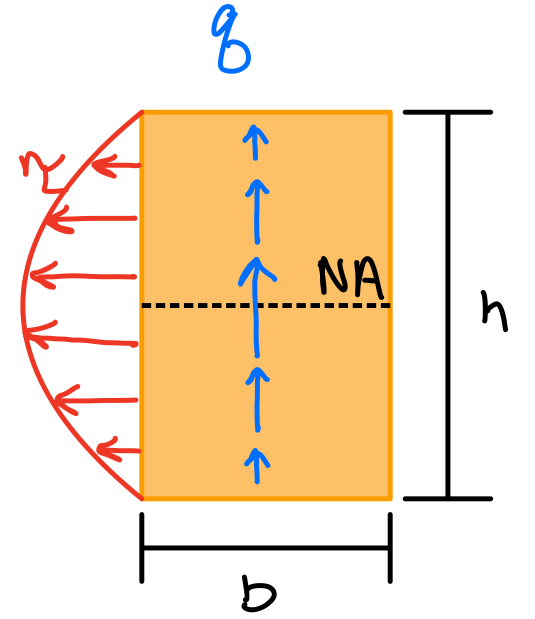
\includegraphics[angle=0, width=2in]{TransverseShear-Figures/ShearFlow.png}
\vspace{-2mm}
\caption{\small \cyan{Taken from the web}}
\vspace{-3mm}
\label{Fig:ShearFlow}
\end{figure*}

\noindent \blue{Built-up beams are beams that have been put together with either an adhesive (glue, epoxy, etc) or fasteners (nails, bolts, etc). Calculating \textbf{Shear flow} allows for determining how much adhesive or how often a fastener is needed.} 

\[dF = \frac{VQ}{I}dx\]

\noindent Where shear flow is: \[q = \frac{dF}{dx} = \frac{VQ}{I}\]

\noindent \cyan{\textbf{**Expandable Derivation**}}
\cyan{
\[F_x = \int\sigma_x dA = 0\]
\[\Sigma F_x = F_{x_1} - F_{x_2} + \Delta H\]
\[\Delta H + \int \frac{M_{x_1} y}{I}dA - \int \frac{M_{x_2} y}{I}dA = 0\]
\[\Delta H = \frac{M_{x_1}-M_{x_2}}{I} \int ydA = 0\]
\[\Delta H = \frac{\Delta M}{I} Q = 0\]
\[\frac{\Delta H}{\Delta x} = \frac{\Delta M}{\Delta x} \frac{Q}{I} = 0\]
\[\lim_{x\to 0} \frac{\Delta H}{\Delta x} = \frac{dH}{dx} = q\]
\[q = \frac{dM}{dx} \frac{Q}{I}\]
}
\noindent \cyan{\textbf{**End Derivation**}}

\begin{figure*}[!h]
\centering
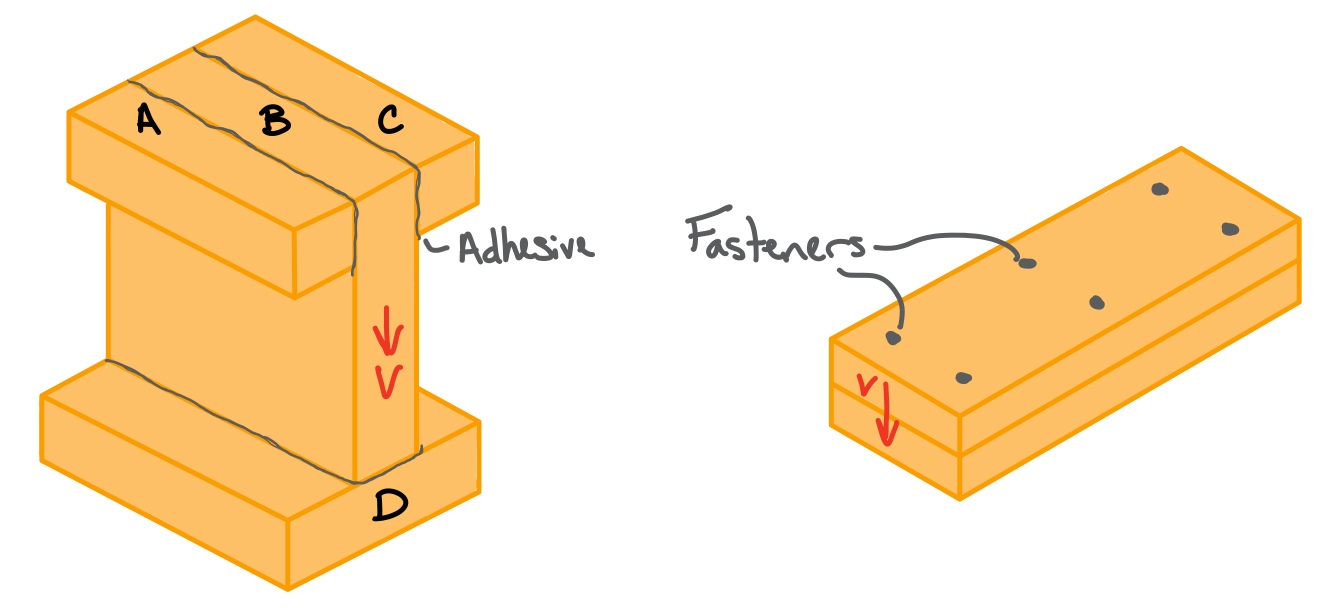
\includegraphics[angle=0, width=4in]{TransverseShear-Figures/BuiltUpBeams.png}
\vspace{-2mm}
\caption{\small \blue{Taken from TAM251 Lecture Notes - L7S13}}
\vspace{-3mm}
\label{Fig:BuiltUpBeams}
\end{figure*}

\subsubsection{\blue{Adhesives}}

\blue{Adhesives supply resistance along the length of the contacting parts. Determine the minimum shear strength at these contacting/weak points using the shear stress equation.}

\subsubsection{\blue{Fasteners}}

\blue{Fasteners supply resistance at fixed intervals. Use the shear flow formula to analyze the beam.}

\subsection{Shear Stresses in Thin-Walled Members \cyan{BSM: not covered in TAM251, not sure if/when it is covered in ME curriculum.}}

\noindent \textbf{\red{**Reference pages have a broken link image here 
 x2**}} 
 
\vspace{5pt}

\noindent The variation of shear flow across the section depends only on the variation of the first moment.
\[q = \tau t = \frac{VQ}{I}\]

\vspace{5pt}

\noindent For a box beam, q grows smoothly from zero at A to a maximum at C and C’ and then decreases back to zero at E.

\vspace{5pt}

\noindent \textbf{\red{**Reference pages have a broken link image here**}}
 
\vspace{5pt}

\noindent  For a wide-flange beam, the shear flow increases symmetrically from zero at A and A’, reaches a maximum at C and then decreases to zero at E and E’.

\vspace{5pt}

 \noindent \textbf{\red{**Reference pages have a broken link image here**}}
